\section{Разработка и внедрение в эксплуатацию}

\subsection{Предобработка и первичный анализ данных}

Используемые данные были собраны из базы данных ClickHouse.
Период собранных данных: от 2 февраля по 11 июня 2020 года.
Данные представляют собой набор около миллиона строк в JSON формате,
которые имеют следующие признаки:

\begin{itemize}
    \item состояние (state) -- категориальный признак, отображающий состояние станка;
    \item оператор станка (operator) -- ФИО оператора станка, выполняющего работы в момент $t$;
    \item название программы (program) -- название запущенной программы;
    \item режим работы лазера (mode), например, автоматический или ручной;
    \item ампераж (amperage);
    \item вольтаж (voltage);
    \item счетчик металлических листов (sheet counter);
    \item температура лазера;
    \item мощность лазера;
    \item установленная мощность лазера;
    \item время в Unix формате.
\end{itemize}

Основными анализируемыми параметрами являются: время,
мощность и температура лазера, установленная мощность лазера.
На момент сбора данных не было возможности
собирать данные по вольтажу и амперажу,
поэтому значения в этих параметров нулевые.
Также не было возможности взятия статистики
по ошибкам программ, так как все ошибки записывались
в связи с запущенными программами.
Данные проблемы будут решены в последующих разработках.

\subsubsection{Проверка на нормальность}

Первым этапом анализа была проверка распределений,
генерируемых временные ряды, на близость к нормальному.
Для этого использовался K-квадрат тест д'Агостина,
который позволяет определить меру сходимости исходого распределения к нормальному.
Гипотеза $H_0$ заключалась в том, что заданное распределение не является нормальным.
Для этого использовалась оценка p-значения.

\begin{figure}[H]
    \center{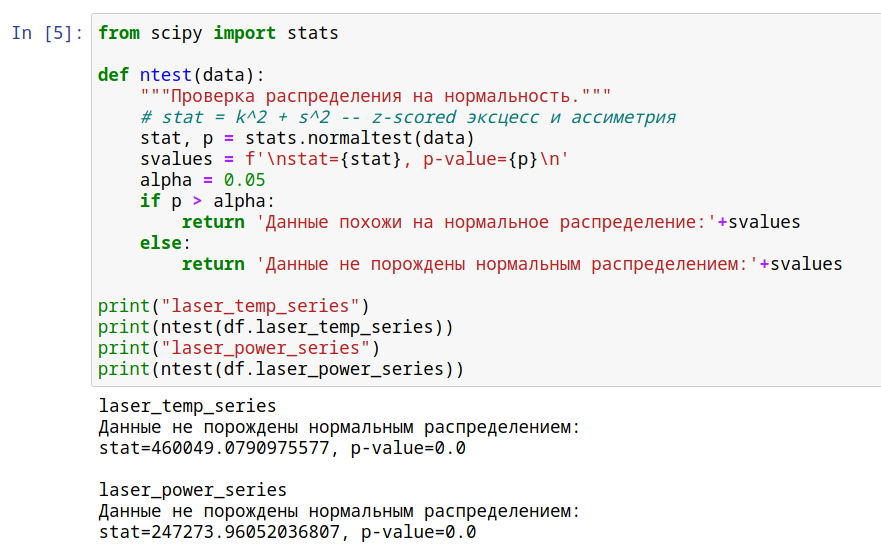
\includegraphics[width=14cm]{normaltest.png}}
    \caption{Тестирование распределений температуры и мощности лазера}
    \label{normaltest}
\end{figure}

Из рисунка \ref{normaltest} видно, что распределения температуры и мощности
не имеют нормальную структуру.

Для более точного представления структуры данных
были вычислены коэффициенты эксцесса и асимметрии.

\begin{figure}[H]
    \center{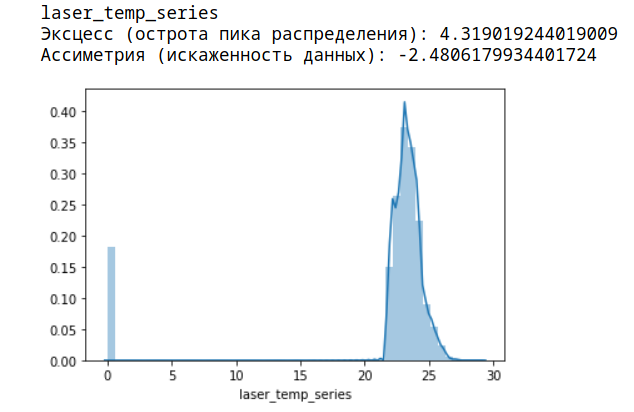
\includegraphics[width=13cm]{tempstruct.png}}
    \caption{Проверка структуры распределения температуры лазера}
    \label{tempstruct}
\end{figure}

\begin{figure}[H]
    \center{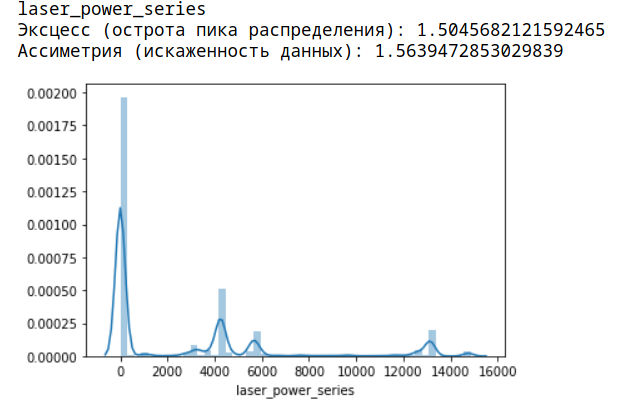
\includegraphics[width=13cm]{powerstruct.png}}
    \caption{Проверка структуры распределения мощности лазера}
    \label{powerstruct}
\end{figure}

На рисунках \ref{tempstruct} и \ref{powerstruct} отображены данные по структуре распределений
температуры и мощности лазера.
Видно, что структура у обоих распределений комплексная,
состоящая из смеси распределений с нетривиальными свойствами.

\subsubsection{Анализ трендов}

На рисунке \ref{trends} видно, что в основном
имеют устойчивый тренд по месяцам.
Дисперсия данных температуры лазера невысокая.

\begin{figure}[H]
    \center{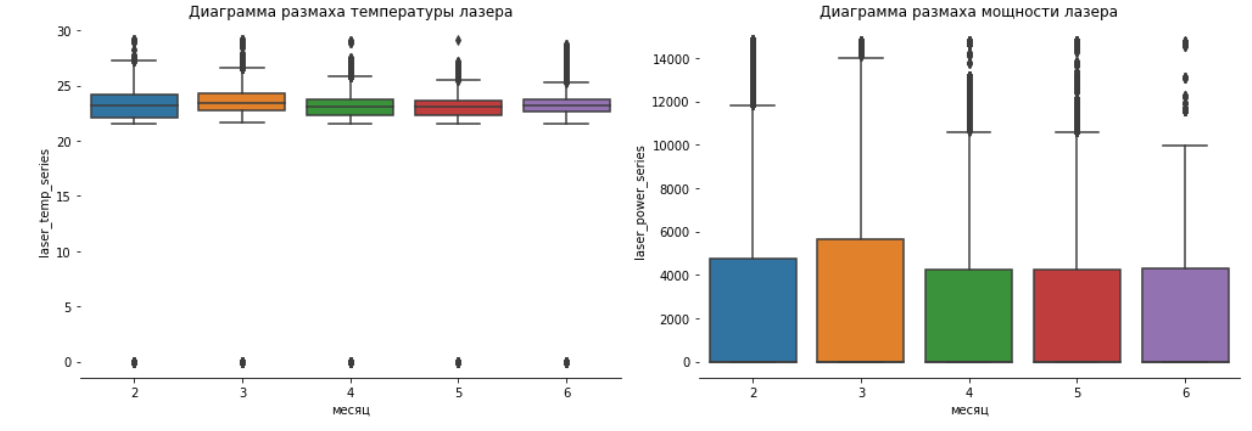
\includegraphics[width=15cm]{trends.png}}
    \caption{Диаграммы размаха}
    \label{trends}
\end{figure}

На рисунках \ref{tempdiv} и \ref{powerdiv} отображены
тренды по дням, неделям и месяцам.
Заметно, что тренд мощности лазера уменьшается.
Это говорит о том, что лазерная голова
станка начинает изнашиваться,
поэтому данный тренд необходимо отслеживать.

\begin{figure}[H]
    \center{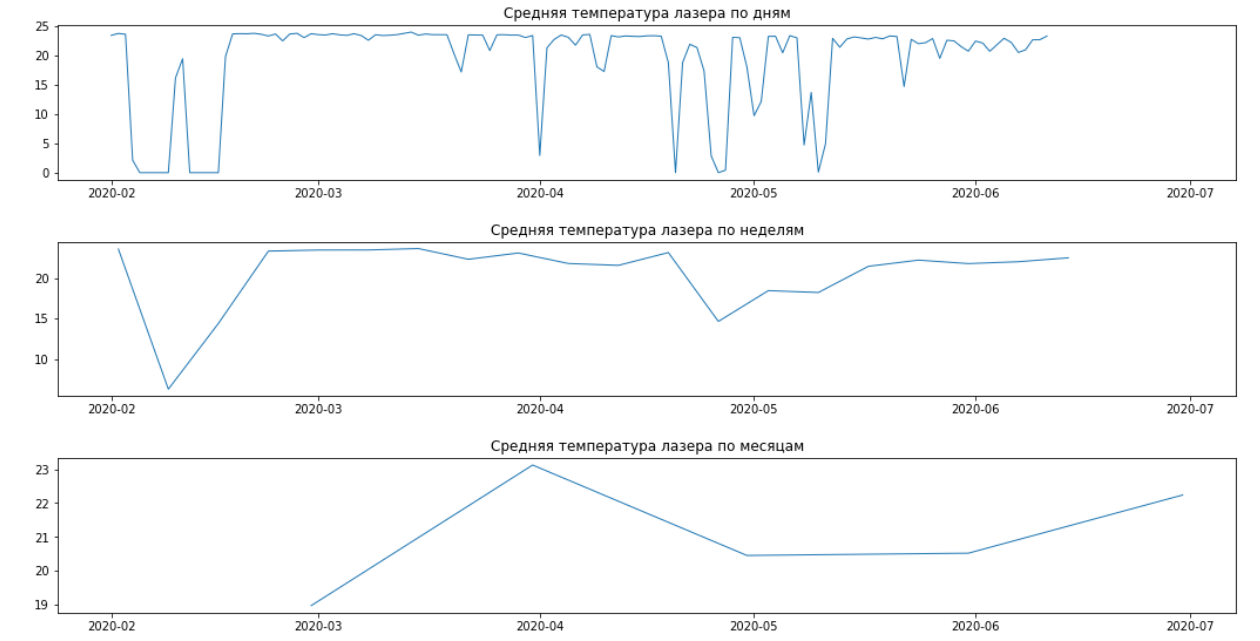
\includegraphics[width=15cm]{tempdiv.png}}
    \caption{Тренды температуры лазера}
    \label{tempdiv}
\end{figure}

\begin{figure}[H]
    \center{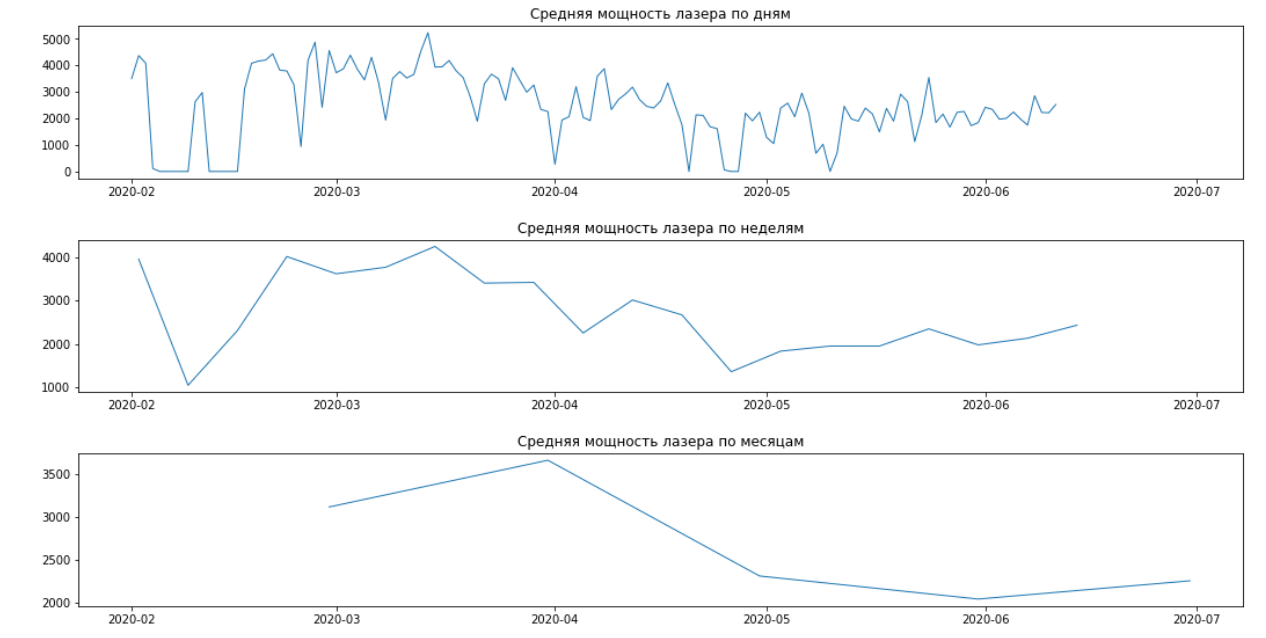
\includegraphics[width=15cm]{powerdiv.png}}
    \caption{Тренды мощности лазера}
    \label{powerdiv}
\end{figure}


На риунке \ref{checkpower} отображены временные
ряды за короткие период двух параметров: фактическая и установленная мощность.
Видно, что установленная мощность постоянна, однако ее могут изменять.
Инженеры компании ВНИТЭП также рекомендуют следить
за регулярным превышением фактической мощности,
что может привести к более быстрому износу,
однако, как уже было описано,
тренд мощности пока только падает.
Для системы предупреждения важно обозначить требования,
на основе которых позволялось использовать мощность
лазера выше установленной в течение какого-то интервала времени.


\begin{figure}[H]
    \center{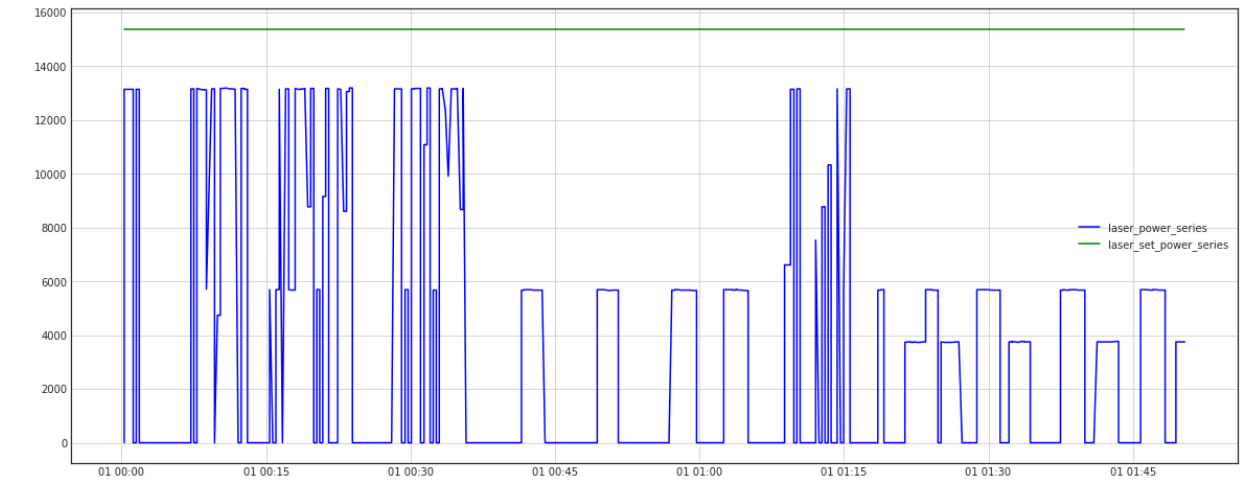
\includegraphics[width=15cm]{checkpower.png}}
    \caption{Фактическая и установленная мощность}
    \label{checkpower}
\end{figure}


Рисунок \ref{powertemp} представляет собой отображение
очевидной связи между мощностью и температурой лазера.
Данные на рисунке нормализованы для наглядного сравнения.

\begin{figure}[H]
    \center{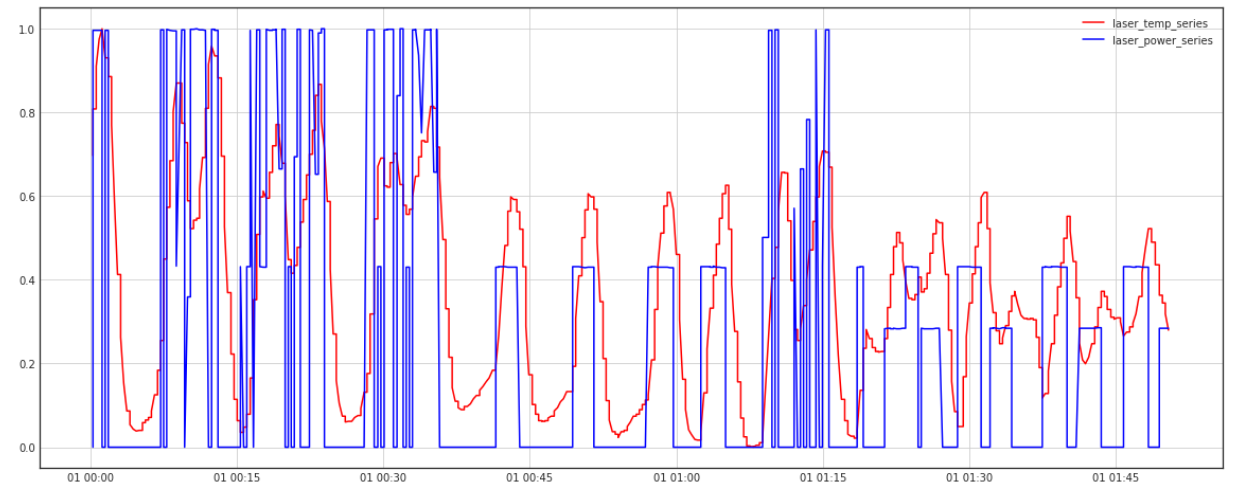
\includegraphics[width=15cm]{powertemp.png}}
    \caption{Отношение температуры и мощности лазера}
    \label{powertemp}
\end{figure}


\subsubsection{Тестирование на стационарность}

Для того, чтобы всецело использовать дальнейшие более сложные методы,
необходимо узнать то, являются ли исследуемые
временные ряды стационарными.
Именно стационарность позволяет
более эффективно работать с временными рядами.
Для этого можно использовать тест Дики-Фуллера.
Данный тест позволяет определить меру того,
насколько данный временной ряд является стационарным.

\begin{figure}[H]
    \center{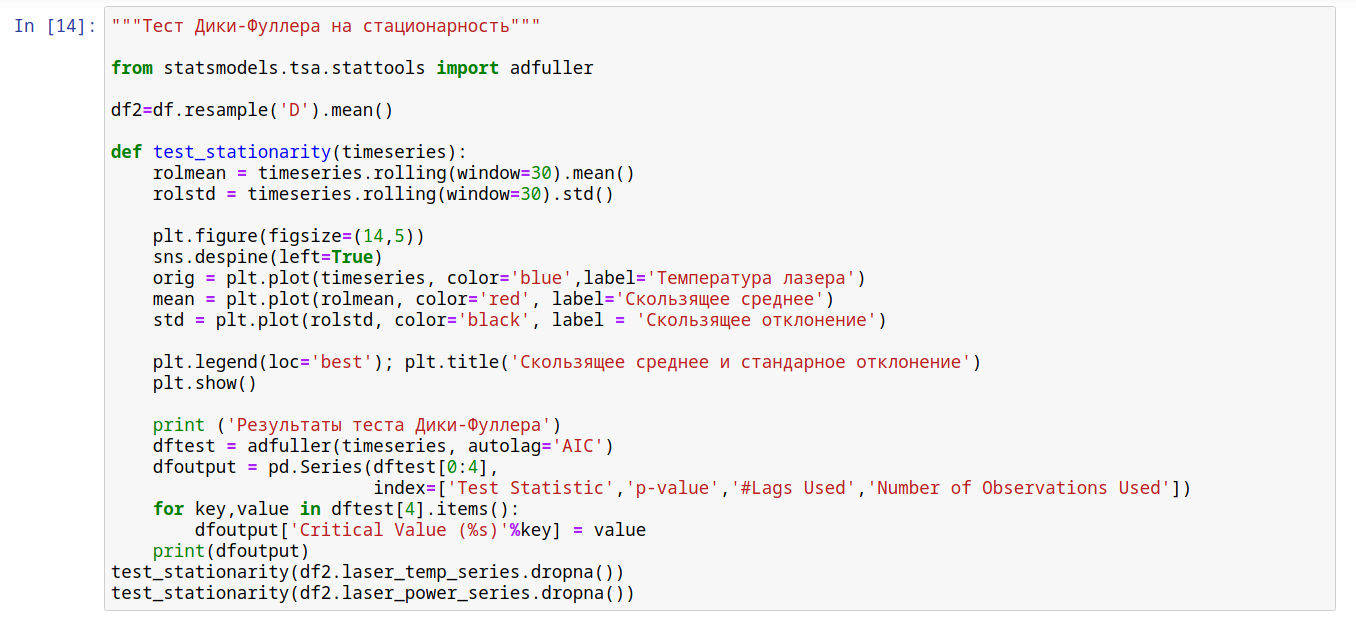
\includegraphics[width=15cm]{fuller.png}}
    \caption{Код для теста Дики-Фуллера}
    \label{fuller}
\end{figure}

На рисунке \ref{fuller} отображен код,
в котором анализируются два временных ряда температуры и мощности лазера на стационарность.
Оба ряда усреднены по дням.

\begin{figure}[H]
    \center{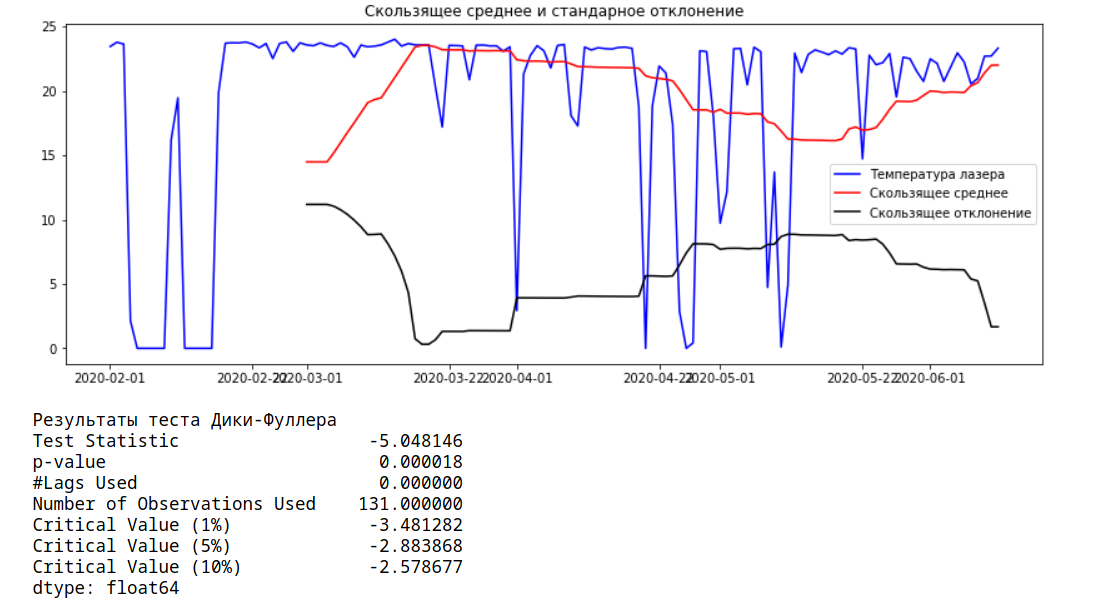
\includegraphics[width=15cm]{fullertemp.png}}
    \caption{Результаты теста для температуры лазера}
    \label{fullertemp}
\end{figure}

\begin{figure}[H]
    \center{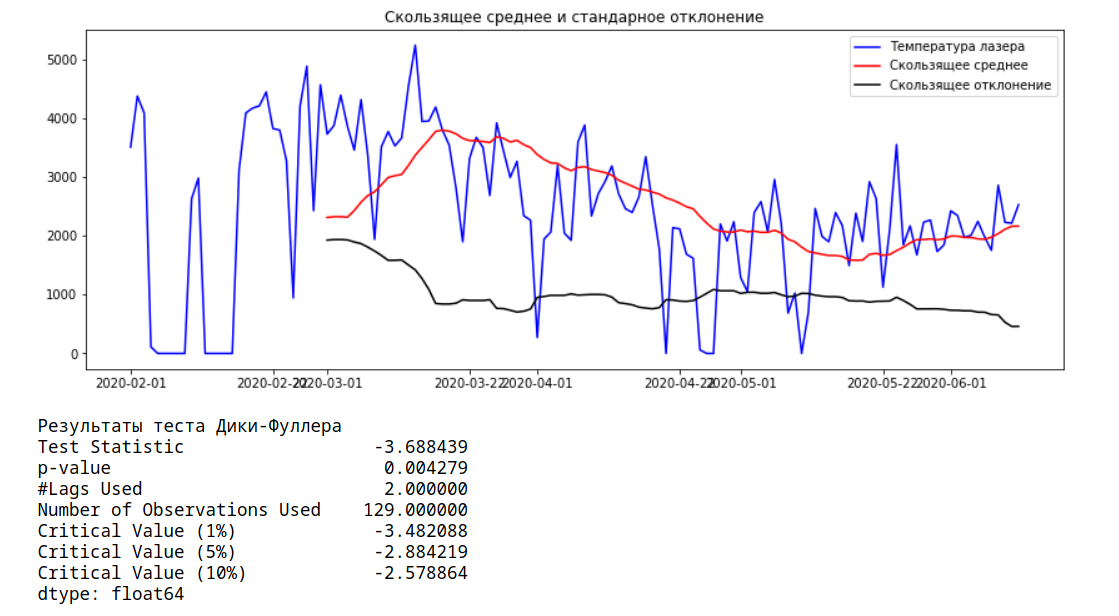
\includegraphics[width=15cm]{fullerpower.png}}
    \caption{Результаты теста для мощности лазера}
    \label{fullerpower}
\end{figure}

\subsection{Архитектура разработанного решения}

(диаграмма пайплайна)


\subsection{Обучение LSTM}

(Оптимальное историческое окно обучения)

(Адаптивное окно предсказания и оптимальные окна обучения)

(диаграмма с окнами)

Обучение моделей на временных рядах может происходить различными способами.
Основным способ является обучение на основе скользящего окна.
Предположим, что есть временной ряд $TS = \{x_1, ..., x_n\}$.
Тогда, скользящим окном называется фрагмент ряда $TS$ размера $m$ с шагом $s$.
Тем самым, исходный ряд разбивается на сегменты одинакового размера: $TS = \{S_1, ..., S_{\frac{n}{s}}\}$.

(LSTM описание)

(кросс-валидация, оценка и прочее)

\subsection{Кластеризация на основе k-Shape}

(оптимальное число кластеров)

(кластеризация)

(описание паттернов)

\subsection{Градиентный бустинг}

(обучение на основе кластеров)

(кросс-валидация)

(тестирование и оценка)

\subsection{Статические критерии}

(описание самостоятельных критериев на основе трендов)

\subsection{Введение в эксплуатацию}

(система оповещения)

(интеграция с omniprocessing и соединение моделей)

(Kuberntetes развертывание)



\clearpage